\chapter{Related work and data employed} \label{chap3}

\section{Related work} \label{3relatedwork}

\subsection{PhysioNet/Computing in Cardiology Challenge 2020}

\subsubsection{Introduction and keypoints}

As I am going to use \cite{physionet_challenge_2020} PhysioNet/Computing in Cardiology Challenge 2020 dataset. It is often good to consider and find out what papers have been published and what kind of architecture they were following. 

\cite{main_arythmia_detection}To encourage more multidisciplinary researches, PhysioNet in Cardiology Challenge 2020 (Challenge 2020) \cite{physionet_challenge_2020} provided high-quality 12-lead ECG data obtained from multiple centers with a large set of cardiac abnormalities. The aim of Challenge 2020 was to identify clinical diagnoses from 12-lead ECG recordings, providing an opportunity to employ various advanced methods to address clinically important questions that are either unsolved or not well-solved \cite{arythmia_detection_9}.

Later I did the specific analysis specifically considering the papers published during the conference. 41 teams got selected during this challenge and others are simply discarded because the method did not work on the hidden set, the team failed to submit a preprint or a final article on time, or the team was absent during the CinC conference. Looking at the 41 teams' papers published in PhysioNet \cite{physionet_challenge_2020}. One can observe that some techniques are used by the majority of the teams. The results indicate that ECG classification is a complex process that includes multiple techniques. Among these techniques, signal processing, DNNs, convolutional neural networks (CNNs), and end-to-end and multi-binary classifications are used by all of the top 10 teams. In addition, there are several important points 1) deep-learning methods were more popular than traditional methods in Challenge 2020; 2) all the teams that employed deep-learning methods used CNNs; and 3) none of the top-10 teams used hand-labelled features (except demographic features); they all adopted end-to-end models instead. 

To investigate the techniques applied by each team, I considered five aspects of the methods that formed a solution pipeline (see \ref{fig:meta_analysis_2020_teams}): data preprocessing, feature engineering, machine-learning models, training strategy, and applications to the real world. Table 2 presents these five aspects.


\begin{figure}[H]
\centering
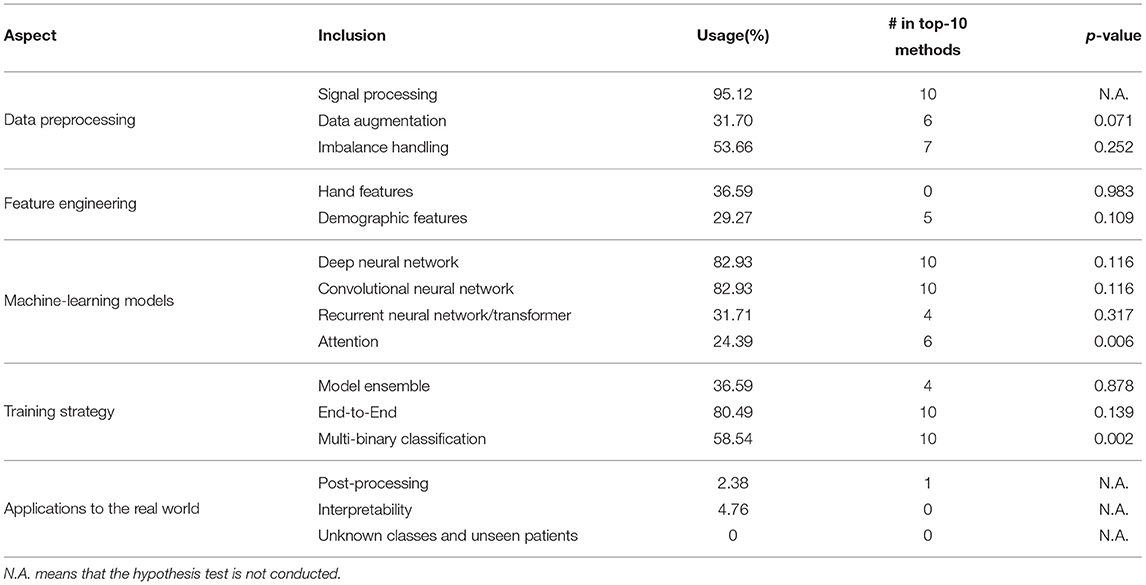
\includegraphics[scale=0.32]{img/meta_analysis_2020_teams.jpeg}
\caption{Details of employed techniques.}
\label{fig:meta_analysis_2020_teams}
\end{figure}


\cite{main_arythmia_detection} One can also notice that the three highest-ranking teams used the model ensemble \cite{first_team, second_team, third_team}, but only 14 out of 41 teams employed this strategy. It is also important to note that model ensemble only helps if used for a single model rather than models that are structurally different. Most of the team also used only age and sex as features rather other using demographic features or 12-lead ECG-based features. The training data in Challenge 2020 suffer from heavy class imbalance (as shown in \ref{fig:label_ditro_alldata}) so most teams used  threshold optimization \cite{eighth_team, second_team, ninth_team} and weighted loss \cite{sixth_team, seventh_team} to handle imbalance class issue. In addition, over-sampling \cite{thirteen_team}, down-sampling \cite{sixteen_team}, and other methods have been employed in Challenge 2020.

\subsubsection{Practical Lessons:}

\begin{enumerate}
  \item Data augmentation should be employed and adapted to specific scenarios.
  \item Combining different features can improve performance.
  \item A hybrid design of different types of deep neural networks (DNNs) is better than using a single type.
   \item The use of end-to-end architectures should depend on the task being solved.
   \item Multiple models are better than one.
\end{enumerate}

\subsubsection{Finding open source algorithms from published papers}

To find the open source code of the papers I searched them on Google and Github, I was able to find the source code of 9 papers that were accepted during the challenge including team 2, team 6 and team 20. I will be later using these source codes for analysis to try to incorporate some additional features that I have identified during the centralized learning approach of Federated learning. 

It is important to note that \textbf{Pytorch} is the most widely used framework by participants implementation of the Physionet Challenge 2020. [\ref{fig:framework_used_by_2020_teams}]. 'Not Mentioned' either represents that they didn't write in their paper what kind of implementation they are following or I am not able to find out their implementation of the paper on the internet. 

\begin{figure}[H]
\centering
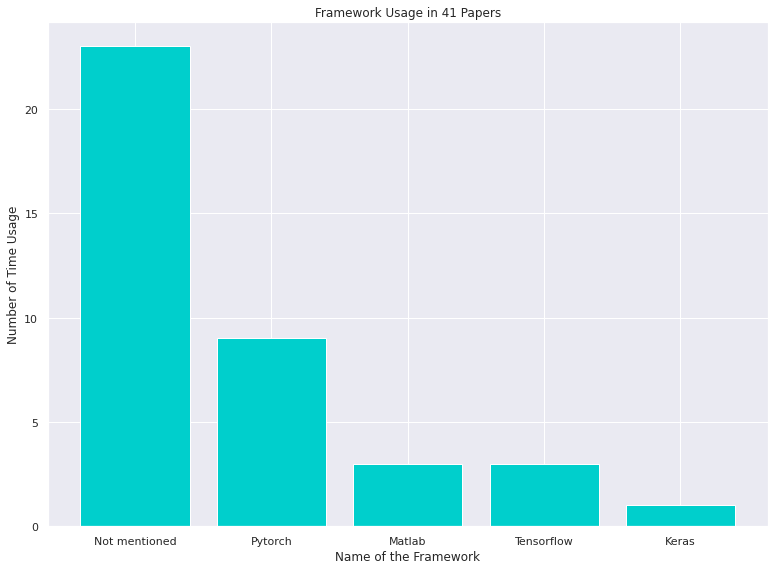
\includegraphics[scale=0.5]{img/framework_usage_in_papers.png}
\caption{Most used framework during Physionet Challenge 2020}
\label{fig:framework_used_by_2020_teams}
\end{figure}

I have also created an excel sheet that has the combination of the meta-analysis of the 2020 challenge \cite{main_arythmia_detection} and all the open source code related to each team that participated in the challenge. Which can be found here: https://bit.ly/3bgFtWs 


\section{Data employed} \label{5dataset}


PhysioNet presents an annual series of biomedical 'Challenges' that focus on unsolved clinical and basic science challenges in collaboration with the annual Computing in Cardiology (CinC) conferences. The National Institutes of Health (NIH), Google, MathWorks, and the Gordon and Betty Moore Foundation have all lent their support to these challenges. George Moody, of the Laboratory for Computational Physiology (LCP), directed these Challenges for the first 15 years (from 2000 to 2014), before retiring due to ill health. Gari Clifford of Emory University and the Georgia Institute of Technology have been leading the Challenges since 2015. In 2021, the ‘PhysioNet/Computing in Cardiology Challenges’ was renamed the ‘George B. Moody PhysioNet Challenges’ to honour George's lifetime contributions to the discipline, particularly his seminal work on the Challenges \cite{dataset1}.

The 2020 Challenge's purpose is to use 12-lead ECG records to detect clinically diagnosis. Starting from the clinical data provided, the participants must implement an open-source algorithm that can automatically classify the
cardiac abnormality or abnormalities present in each 12-lead ECG recording
and provide a probability or confidence score for each of them, with an
emphasis on 27 diagnoses \ref{table:diagnoses_SNOMED} To determine the winner, the trained
models of the participants are run on hidden validation and test sets and
their performance is evaluated using a novel, expert-based evaluation
metric designed specifically for the 2020 Challenge. The team whose
the algorithm that achieves the highest score is the winner of the Challenge.

\newpage 


\begin{table}[H]
\begin{center}
\begin{tabular}{|c | c | c |}
 \hline
\textbf{Diagnosis} & \textbf{Code} & \textbf{Abbreviation} \\ [0.4ex] 
\hline \hline
1st degree AV block  & 270492004 & IAVB \\ \hline
Atrial fibrillation  & 164889003 & AF \\ \hline
Atrial flutter  & 164890007 & AFL \\ \hline
Bradycardia  & 426627000 & Brady \\ \hline
Complete right bundle branch block  & 713427006 & CRBBB \\ \hline
Incomplete right bundle branch block  & 713426002 & IRBBB \\ \hline
Left anterior fascicular block  & 445118002 & LAnFB \\ \hline
Left axis deviation  & 39732003 & LAD \\ \hline
Left bundle branch block  & 164909002 & LBBB \\ \hline
Low QRS voltages  & 251146004 & LQRSV \\ \hline
Nonspecific intraventricular conduction disorder  & 698252002 & NSIVCB \\ \hline
Pacing rhythm  & 10370003 & PR \\ \hline
Premature atrial contraction  & 284470004 & PAC \\ \hline
Premature ventricular contractions  & 427172004 & PVC \\ \hline
Prolonged PR interval  & 164947007 & LPR \\ \hline
Prolonged QT interval  & 111975006 & LQT \\ \hline
Q wave abnormal  & 164917005 & QAb \\ \hline
Right axis deviation  & 47665007 & RAD \\ \hline
Right bundle branch block  & 59118001 & RBBB \\ \hline
Sinus arrhythmia  & 427393009 & SA \\ \hline
Sinus bradycardia  & 426177001 & SB \\ \hline
Sinus rhythm  & 426783006 & NSR \\ \hline
Sinus tachycardia  & 427084000 & STach \\ \hline
Supraventricular premature beats  & 63593006 & SVPB \\ \hline
T wave abnormal  & 164934002 & Tab \\ \hline
T wave inversion  & 59931005 & TInv \\ \hline
Ventricular premature beats  & 17338001 & VPB \\ \hline

\hline\hline
\end{tabular}
\end{center}
\caption{Diagnoses, SNOMED CT codes and abbreviations for the 27 diagnoses that were scored for the Challenge.}
\label{table:diagnoses_SNOMED}
\end{table}

The data are from five different sources:
\begin{enumerate}
    \item CPSC Database and CPSC-Extra Database
    \item INCART Database
    \item PTB and PTB-XL Database
    \item The Georgia 12-lead ECG Challenge (G12EC) Database 
    \item Undisclosed Database
\end{enumerate}

The first source consists of three databases from the China Physiological Signal Challenge 2018 (CPSC2018), which took place in Nanjing, China at the 7th International Conference on Biomedical Engineering and Biotechnology \cite{dataset2}: the original public training dataset (CPSC), an unused dataset (CPSC-Extra), and the test dataset (the hidden CPSC set). The first two were shared as training sets, while the last one was split into validation and test sets for the 2020 Challenge. This training set consists of two sets of 6,877 (male: 3,699; female: 3,178) and 3,453 (male: 1,843; female: 1,610) of 12-15 ECG recordings lasting from 6 seconds to 60 seconds. Each recording was sampled at 500 Hz.

The second source is the public dataset from the St. Petersburg Institute of Cardiological Technics (INCART) 12-lead Arrhythmia Database [15 V. Tihonenko, A. Khaustov, S. Ivanov, A. Rivin, and E. Yakushenko, “St Petersburg INCART 12-lead arrhythmia database”, PhysioBank, PhysioToolkit, and PhysioNet, 2008, DOI: 10.13026/C2V88N.]. The dataset was shared as a training set. This database consists of 74 annotated recordings extracted from 32 Holter records. Each record is 30 minutes long and contains 12 standard leads, each sampled at 257 Hz.

The third source from the Physikalisch Technische Bundesanstalt (PTB) includes two public databases which were shared as training sets: the PTB Diagnostic ECG Database and the PTB-XL, a large publicly available electrocardiography dataset. The first PTB database contains 516 records (male: 377, female: 139). Each recording was sampled at 1000 Hz. The PTB-XL contains 21,837 clinical 12-lead ECGs (male: 11,379 and female: 10,458) of 10-second length with a sampling frequency of 500 Hz.


The fourth source is the Georgia 12-lead ECG Challenge (G12EC) Database. This is a new database, representing a large population from the Southeastern United States, and is split between the training, validation, and test sets. The validation and test set comprised the hidden G12EC set. This training set contains 10,344 12-lead ECGs (male: 5,551, female: 4,793) of 10-second length with a sampling frequency of 500 Hz.

The fifth source is a dataset from an undisclosed American institution that is geographically distinct from the other dataset sources. This dataset has never been posted publicly and contains 10,000 ECGs all retained as test data \cite{dataset2}. As the mentioned dataset was not disclosed, I didn't use that one in my experiments.

The actual count of all the diagnoses by each database can be found in Figure \ref{fig:diagnose_count_by_db}. That was obtained by taking the first arrhythmia reported by each recording since each patient could contain more than one diagnosis based on its ECG.

\begin{figure}[H]
\centering
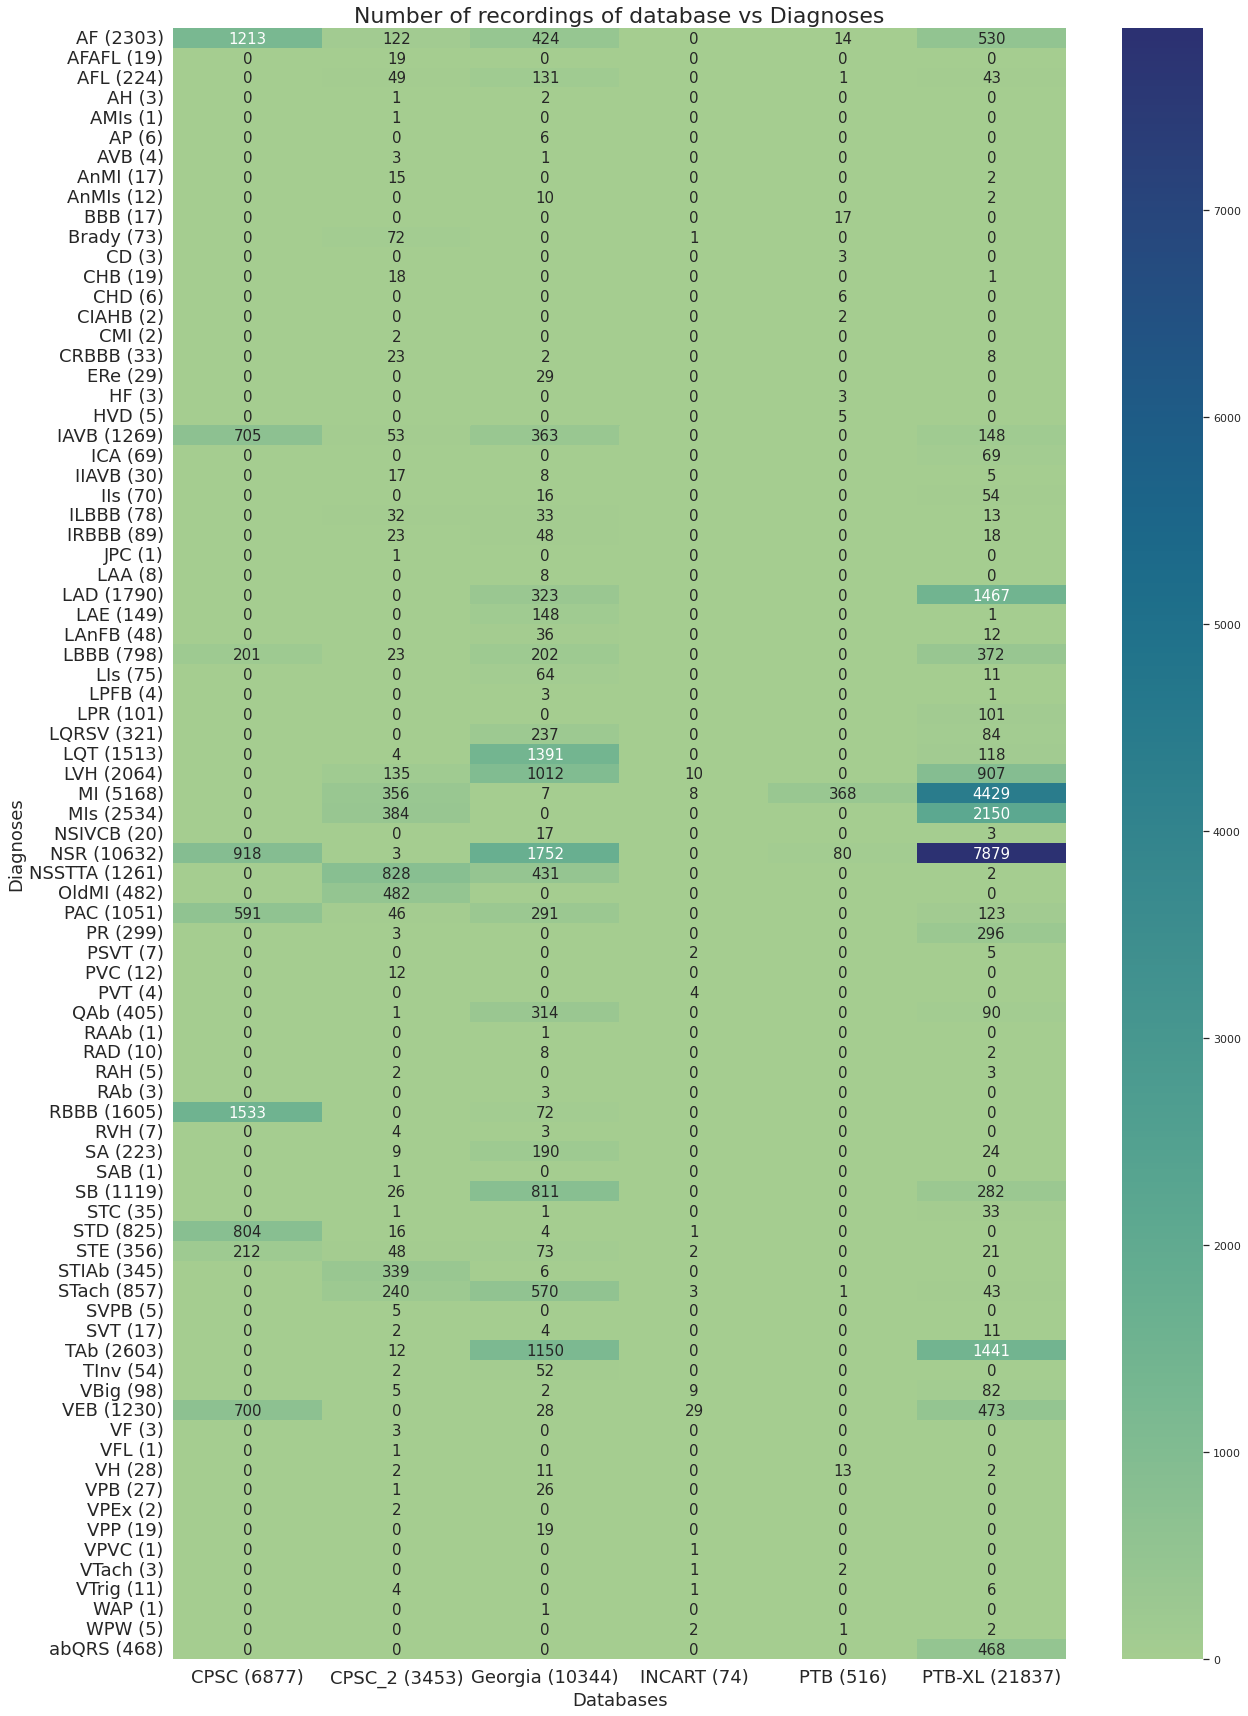
\includegraphics[scale=0.3]{img/diagnose_count_by_db.png}
\caption{Number of recordings for each diagnosis by database}
\label{fig:diagnose_count_by_db}
\end{figure}

All data is provided in WFDB format. Each ECG recording has a binary \textbf{MATLAB v4 file} for the ECG signal data and a \textbf{text file} in WFDB header format describing the recording and patient attributes, including the diagnosis \cite{dataset3} \cite{dataset2} \cite{dataset4}.
